\documentclass[a4paper, 11pt]{article}
\usepackage{geometry}
\usepackage{indentfirst}
\usepackage{setspace}
\usepackage{amsmath}
\usepackage{graphicx}
\usepackage{wrapfig}
\usepackage{caption}
\usepackage{indentfirst}
\setlength{\parindent}{20pt}
\usepackage{amssymb}
\usepackage{float}
\usepackage{subcaption}

\graphicspath{ {./images/} }
\geometry{left=2.5cm, right=2.5cm, top=2.5cm, bottom=2.5cm}

\begin{document}	
	\title{Exercise \# 3. Numerical Solution of the Poisson Problem. }
	\author{{\small Alexandre Rodrigues (2039952)}}
	\date{\today}
	
	\maketitle
		\section{Problem statement}
			The aim of this exercise is to solve the following homogeneous boundary value problem.
			Find $u$ such that 
			\begin{align}
				-\frac{\partial^2 u}{\partial x^2} -\frac{\partial^2 u}{\partial y^2} &= f \qquad \qquad &\text{in} \ \Omega \\
				u &= 0 \qquad \qquad & \text{on} \ \Gamma
				\label{eq:prob}
			\end{align}
			valid in the domain $ \Omega = \{ (x,y) : -1 \le x \le , -1 \le y \le 1\} $, $\Gamma = \partial \Omega$ being its boundary.
			
			The term $f$ is:
			\begin{equation}
				f(x,y) = -4 + 2 x^2 + 2 y^2
				\label{eq:f}
			\end{equation}
		
			Only Dirichlet conditions apply so the analytical solution will be:
			\begin{equation}
				u(x,y) = x^2 + y^2 - x^2 y^2 -1
				\label{eq:analytic}
			\end{equation}
		
			This problem will be solved with the Finite Element Method using triangular elements and linear basis functions.
			It can simulate an elastic membrane fixed ate the boundary, with small displacement and an orthogonal force with intensity $ f $.
			The Dirichlet conditions define how the membrane is fixed and $u$ is the out-of-plane displacement of the membrane.
			
		
			\section{Step-by-step Implementation}
				We can reduce the problem to a linear system.
				\begin{equation}
					H \mathbf{u} - \mathbf{f} = 0,
				\end{equation}
				with $ n $ unknowns (vector $ u $), $ n $ being the number of FEM points.
			
			
				Based on the homework text I implemented each of these steps in Matlab.
			
			\begin{enumerate}
				\item \textbf{Input files from specified mesh:} 
				
					All 3 files are loaded: \texttt{topol}, \texttt{bound} and \texttt{coord}, for the current mesh refinement level.	
				
				\item \textbf{Create pattern for the stiffness matrix:} 
					\subitem \textbf{1.} Create a range vector 1 to \texttt{Ne}, then place it 3 times as a column in a matrix and reshape the matrix to obtain the column vector $ row = [1,1,1,2,2,2,3,\ldots]^T $. 
					\subitem \textbf{2.} The \texttt{col} vector is simply obtained by reshaping the \texttt{topol} as a column vector. 
					\subitem \textbf{3.} Compute the adjacency matrix as \texttt{A = sparse(row,col,1)} and the pattern for the stiffness matrix as \texttt{H = A' * A}, finally cleaning the matrix coefficients as we only want the sparse pattern, \texttt{H = H * 0}.
				
				\item \textbf{Compute the stiffness matrix $H$:}
				
					I created the function \texttt{[H, delta] = computeStiff(H, topol, coord)} to encapsulate all the following computations.
					It has the topology and coordinates matrices as inputs, as well as the $ H $ matrix with its pattern already defined before.
					It returns the final $ H $ matrix and the \texttt{delta} vector with the surface measures of each element.
					Using a for loop for each element:
					\subitem \textbf{1.} Get coordinates of the 3 nodes that define the element, compute the surface measure for that element and save it in the \texttt{delta} vector.
					$$ \Delta = \frac{1}{2} \begin{vmatrix} 1 & x_i & y_i \\ 1 & x_j & y_j \\ 1 & x_m & y_m \end{vmatrix} $$
					\subitem \textbf{2.} Compute the $ b $ and $ c  $ coefficients of the basis functions ($a$ is not needed): 
					$$  b_i = y_j - y_m  \qquad c_i = x_m - x_j ,$$ others are obtained using anticlockwise indices permutation.
					\subitem \textbf{3.} Compute \texttt{Hloc} for an element as 
					$$ H_{loc} = \frac{1}{4\Delta}\{ b^Tb + c^Tc \} $$ 
					where $ b = [b_i, b_j, b_m]$ and $ c = [c_i, c_j, c_m]$
					\subitem \textbf{4.} Assemble the stiffness matrix H from the local matrices using algorithm 3.3 of the exercise text.
				
				\item  \textbf{Compute the right hand size $f$ :}
				
					Using a for loop to iterate in the list of nodes:
					\subitem \textbf{1.} Get the node coordinates;
					\subitem \textbf{2.} Find elements that have this node as a vertex and get their surface measures from the \texttt{delta} vector;
					\subitem \textbf{3.} Compute the right hand size vector as $f_i \approxeq (-4 +2x_i^2 + 2y_i^2)  \frac{\sum_e \Delta_e}{3} $
				
				\item \textbf{Enforce the boundary conditions:}
				
					For this problem we can simply substitute the diagonal value of $ H $ at the node \texttt{i} of the boundary with a large enough constant, \texttt{H(i,i) = Rmax}.
					
				
				\item \textbf{Solve the Linear System:}
				
					Following recommendations I used Matlab's PCG method with tolerance $ 1 \times 10^{-8} $, Jacobi preconditioner as \texttt{M = sparse(diag(diag(H)))} and Cholesky preconditioner as \texttt{L = ichol(H)}.
				
				\item \textbf{Error computation:}
				
					 Using a for loop to visit each node:
					\subitem \textbf{1.} Get the coordinates of the node;
					\subitem \textbf{2.} Compute the analytical solution as $u(x,y) = x^2 + y^2 - x^2y^2 - 1$;
					\subitem \textbf{3.} Sum surface measures of each element that have this node as a vertex;
					\subitem \textbf{4.} Compute local error as $ (u_i - u(x_i,y_i))^ 2 \ \frac{\sum_e \Delta_e}{3} $;
					\subitem \textbf{5.} Sum all the local errors and $ \epsilon $ will be its square root.	
			\end{enumerate}
			
					
		\section{Results}
		
			\subsection{Convergence Plots}
			
				The following images show the convergence plots for all refinement levels, one for each preconditioner.
				
				\begin{figure}[H]
					\begin{subfigure}{.49\textwidth}
						\centering
						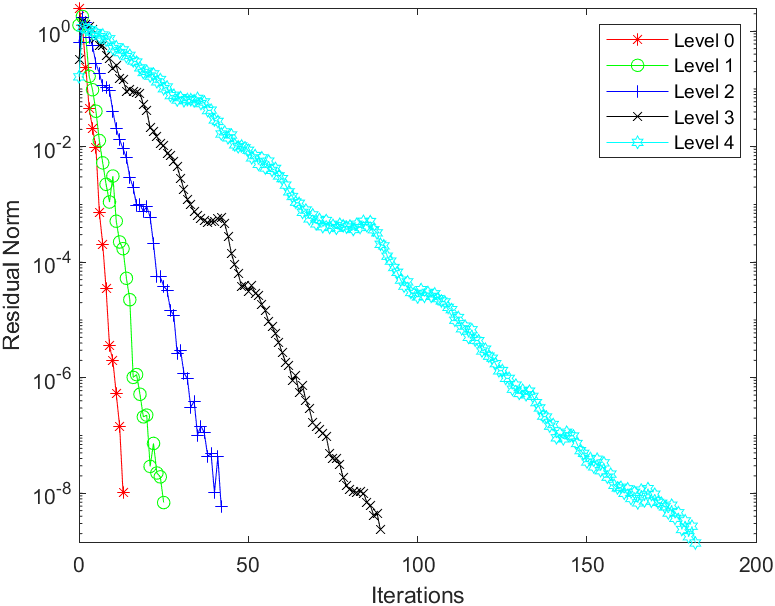
\includegraphics[width=.99\linewidth]{ConvergenceJ.png}  
						\caption{Jacobi}
						\label{fig:Jacobi}
					\end{subfigure}
					\begin{subfigure}{.49\textwidth}
						\centering
						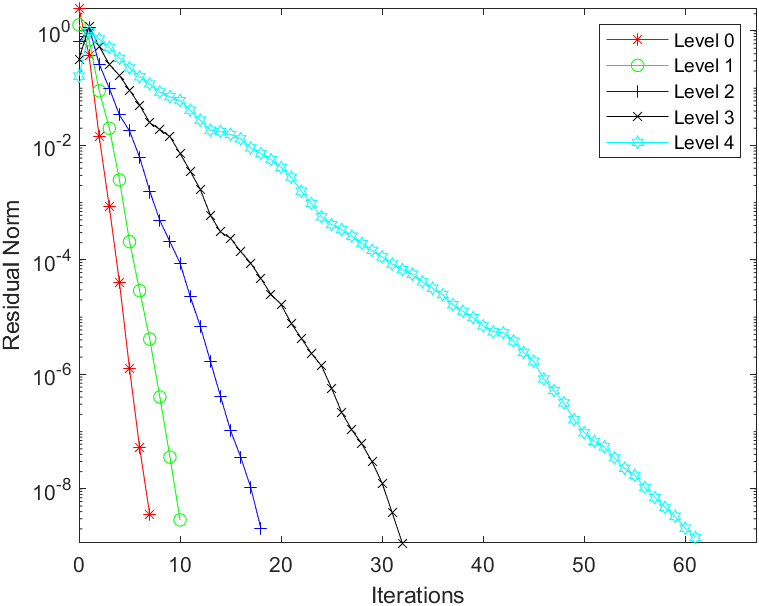
\includegraphics[width=.99\linewidth]{ConvergenceC.png}  
						\caption{Cholesky}
						\label{fig:Chol}
					\end{subfigure}
					\caption{Convergence plots - Residual norms vs. iterations}
					\label{fig:convergence}
				\end{figure}
				
				There are clear differences in convergence regarding the preconditioner used.
				The Cholesky preconditioner significantly improves convergence by reducing the number of iterations needed by up to a factor of 3.
				
				There is also a clear slowdown of convergence when increasing the level of refinement.
				
				These results are as expected, increasing the preconditioner complexity improves efficiency of the PCG and increasing the level of refinement increases complexity of the FEM code and thus requires more computational time.
						
				I also recorded the computational time needed to solve each PCG method but found no relevant differences.
				
			\subsection{Error}
				\begin{table}[H]
					\centering
					\begin{tabular}{c|c|c}         
						\textbf{Level} 	& \textbf{ Error $ \epsilon $} 		& \textbf{Error Ratio}  \\ \hline
						$ 0  $			& $ 6.912 \times 10^{-2} $ 	& N/A \\ \hline
						$ 1  $			& $ 1.631 \times 10^{-2} $ 	& $ 0.236 $ \\ \hline
						$ 2  $			& $ 3.984 \times 10^{-3} $ 	& $ 0.244 $ \\ \hline
						$ 3  $			& $ 9.883 \times 10^{-4} $	& $ 0.248 $ \\ \hline
						$ 4  $			& $ 2.465 \times 10^{-4} $ 	& $ 0.249 $ \\ 
					\end{tabular}
					\caption{FEM Convergence table}
					\label{table:errors}
				\end{table}
				Each level of refinement decreases $ l $ by a factor of $ 2 $, $ l_{i+1} = \frac{1}{2}l_i $.
				The error is proportional to $l^2$ so $ \epsilon_{i+1} = \frac{1}{4}\epsilon_i $.
				So we can conclude that the results are as expected.
			
			\section{Conclusion}
				We can hereby conclude that the Finite Element Method is a good approach to solve these types of problems.
				
				The method converged relatively fast, in less than 1 second.
				Using even more refined meshes would produce smaller errors and still be fast enough, although this does not take into account the mesh computation.
				
				The best results were obtained from the most refined mesh and the Cholesky preconditioner but this scenario is also the slowest to finish when including the factorization.
	
	
\end{document}



